% Generated by `python -m experiments.experiment_3.appendix_captions` -- do not edit by hand.
% Main-text figure for Experiment 3. Needs \usepackage{graphicx}; paths are relative to
% outputs/finals/experiment-3/.
\begin{figure}[tbp]
  \centering
  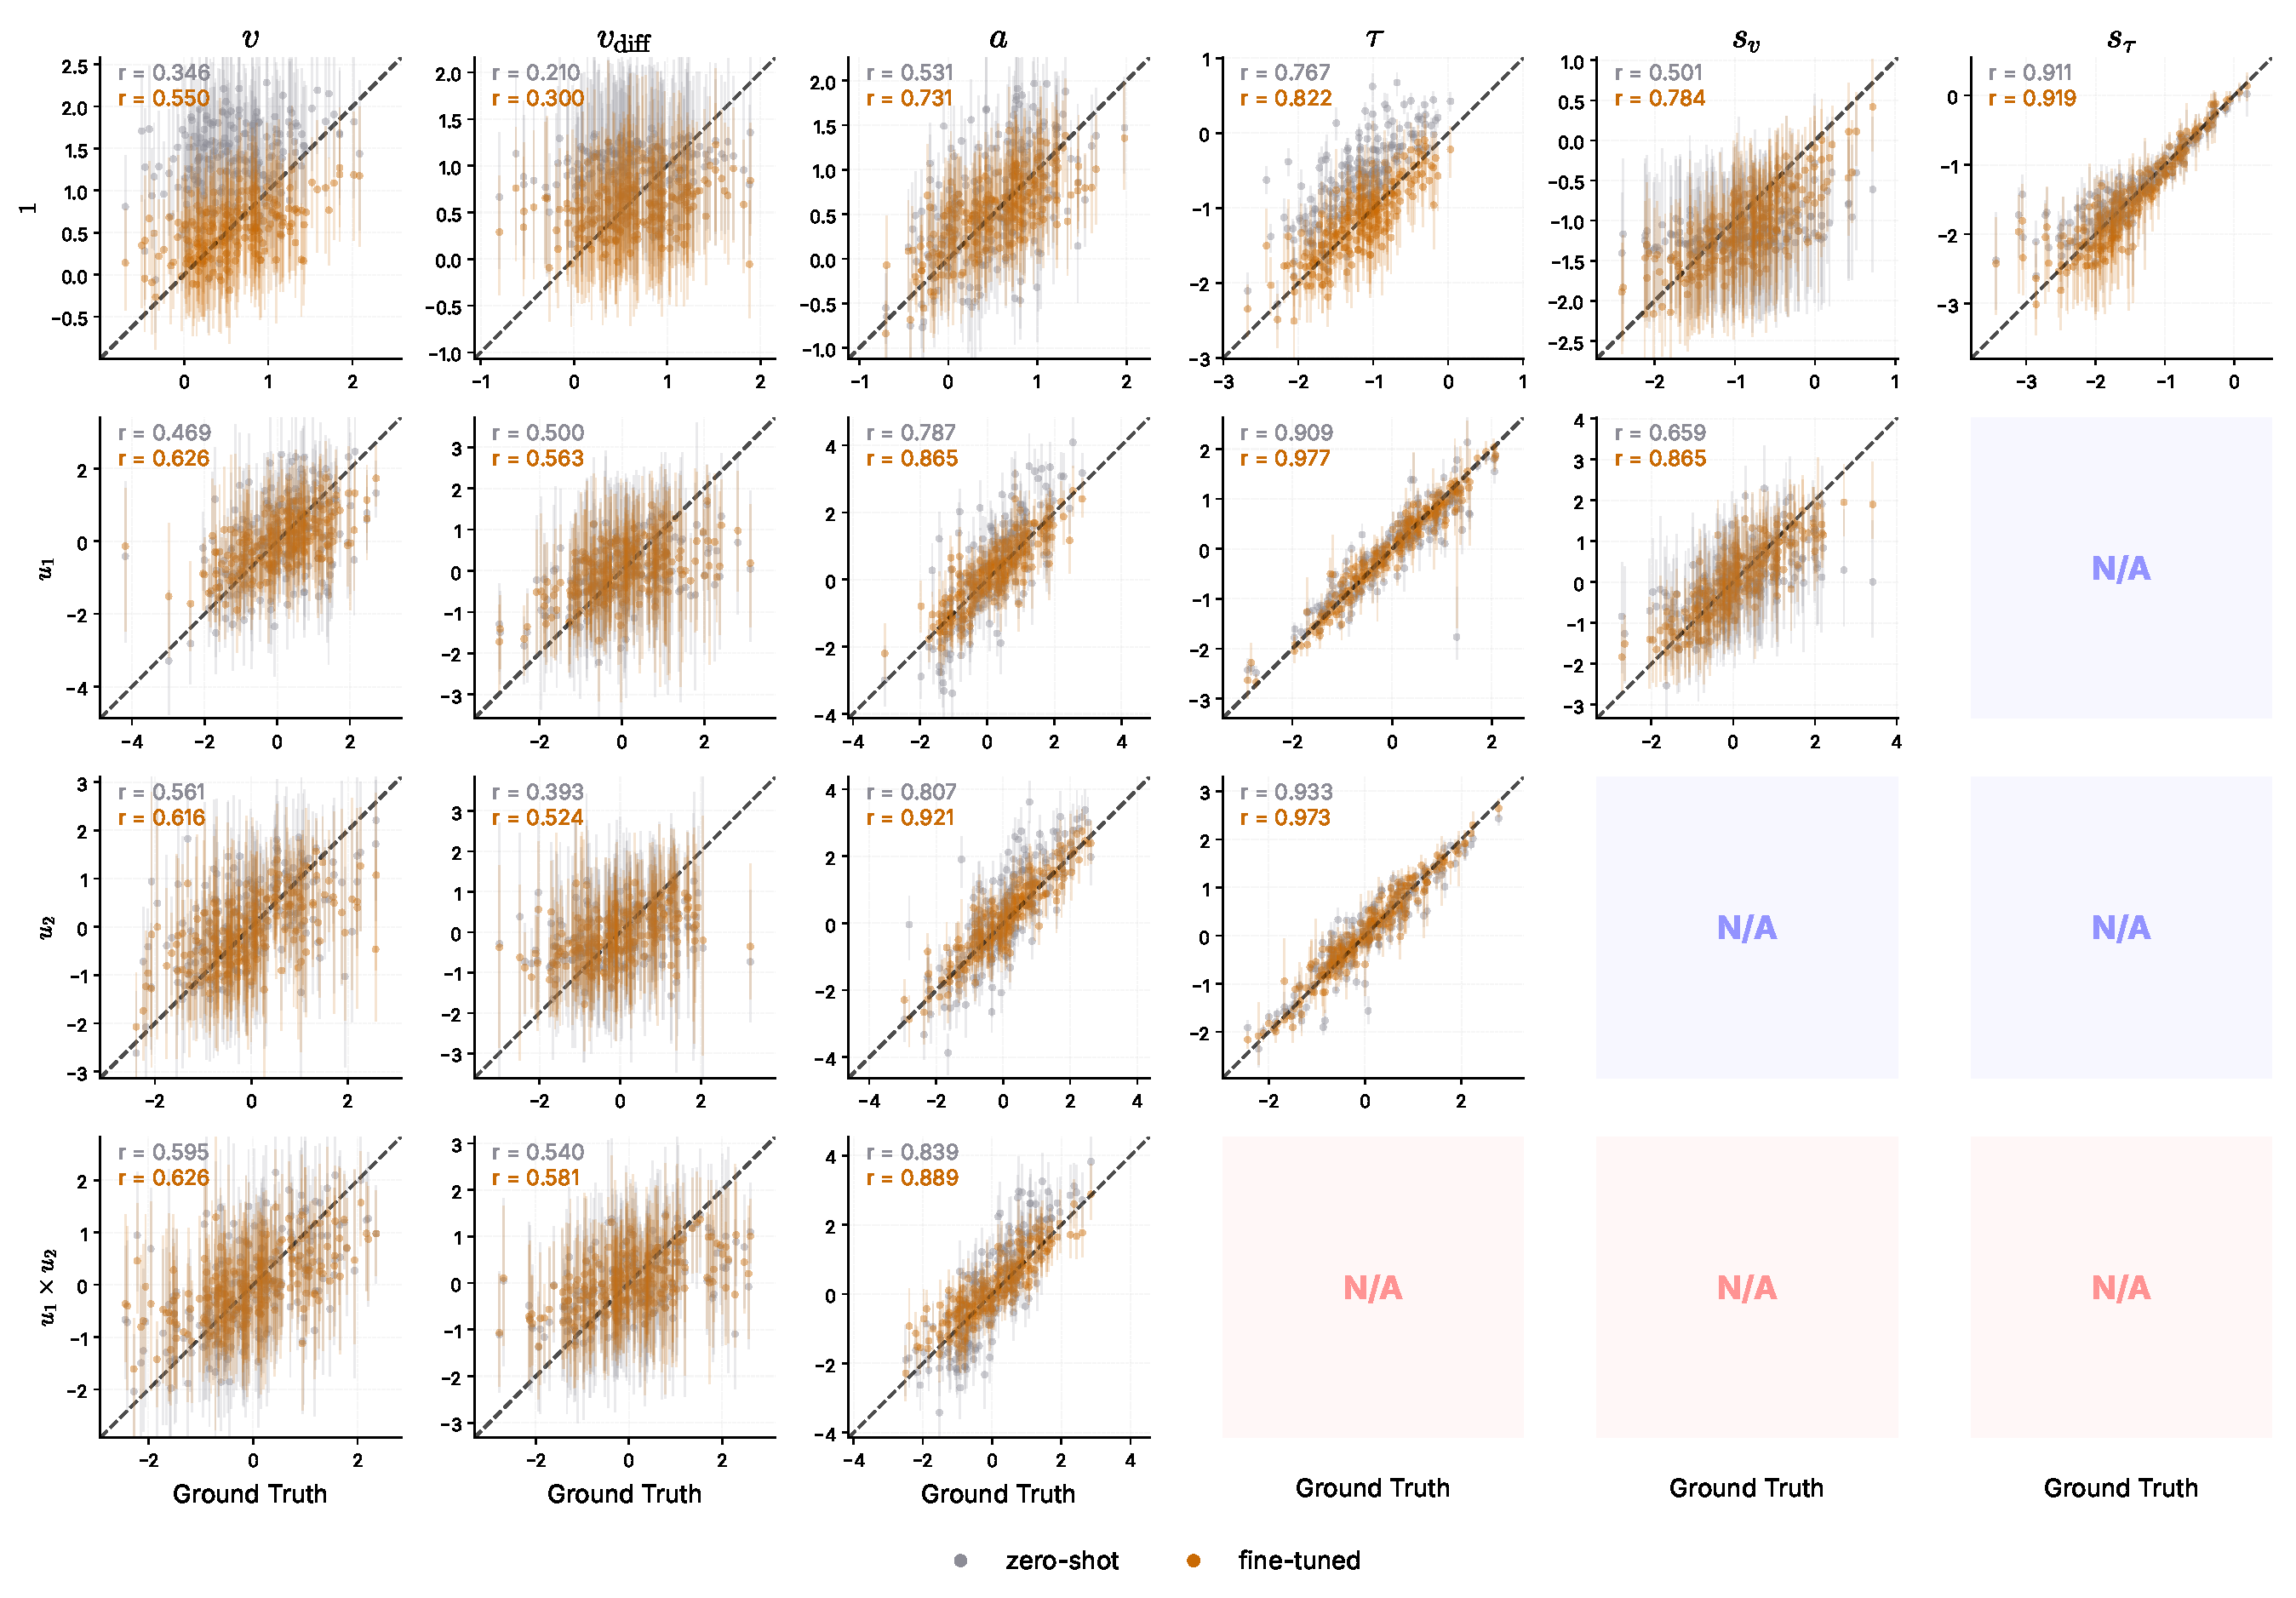
\includegraphics[width=\textwidth]{compare/lba/interaction_overlay_recovery.pdf}\par\vspace{1ex}
  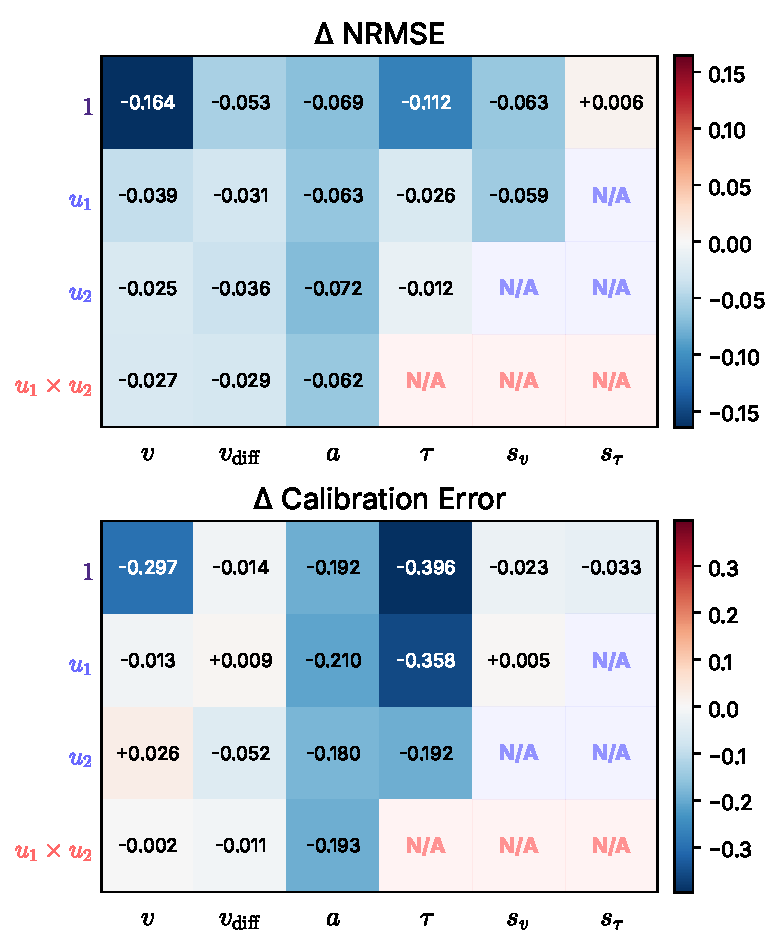
\includegraphics[width=\textwidth]{compare/delta_metrics_interaction.pdf}
  \caption{\textbf{Transfer to a held-out model family.} Top: parameter recovery for the LBA, which was not among the training families, by the original CogFormer network without any LBA training (zero-shot, grey) and by the same network after fine-tuning on all four families (orange), on the same 200 test datasets of the \emph{interaction} design: posterior means against ground truth with 90\% credible intervals, one $r$ per network. Columns are the parameters and rows the coefficients (intercept, slopes on $u_1$ and $u_2$, and on their product); N/A marks coefficients the design does not contain. Bottom: change in each of the LBA's coefficients' NRMSE (top) and calibration error (bottom) with fine-tuning (fine-tuned minus zero-shot), cells laid out as in the top panel. Negative values (blue) are improvements, positive values (red) deteriorations; each panel has its own colour scale. The LBA's largest change in magnitude is 0.164 in NRMSE and 0.396 in calibration error; for DDM, RDM and CDM (fine-tuned minus the original network, not shown) it is 0.005 and 0.051. Details in Appendix~\ref{app:exp3-main-details}.}
  \label{fig:exp3-main}
\end{figure}
